\documentclass{standalone}
\usepackage{tikz}
\usepackage{adjustbox}
\usepackage{verbatim}

\begin{comment}
:Title: \texttt{G4HepEm} libraries and their dependences. 

\end{comment}
\usetikzlibrary{shapes.gates.logic.US,trees,positioning,arrows}

\begin{document}

\begin{adjustbox}{width=10cm, height=6cm, keepaspectratio}
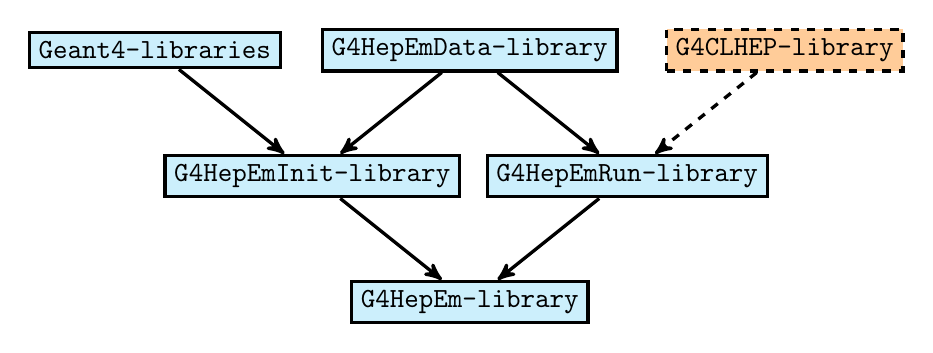
\begin{tikzpicture}
%% Draw system flow diagram
   \begin{scope}[very thick, node distance=1.6cm,on grid,>=stealth',
		lib/.style={rectangle,draw,fill=cyan!20},
		libTmp/.style={rectangle,dashed,draw,fill=orange!40}]
   \node [lib] (HepEm)                                         {\texttt{G4HepEm-library}};
   \node [lib] (HepEmInit)	[above=of HepEm,xshift=-2.0cm]     {\texttt{G4HepEmInit-library}} edge [->] (HepEm);
   \node [lib] (HepEmRun)	  [above=of HepEm,xshift=+2.0cm]     {\texttt{G4HepEmRun-library}}  edge [->] (HepEm);
   \node [lib] (Geant4)	    [above=of HepEmInit,xshift=-2.0cm] {\texttt{Geant4-libraries}}    edge [->] (HepEmInit);
   \node [lib] (HepEmData)	[above=of HepEmInit,xshift=+2.0cm] {\texttt{G4HepEmData-library}} edge [->] (HepEmInit);
   \node [lib] (HepEmData)	[above=of HepEmInit,xshift=+2.0cm] {\texttt{G4HepEmData-library}} edge [->] (HepEmRun);
   \node [libTmp] (G4CLHEP)    [above=of HepEmRun,xshift=+2.0cm]  {\texttt{G4CLHEP-library}}     edge [dashed,->] (HepEmRun);
   \end{scope}
\end{tikzpicture}
\end{adjustbox}%

\end{document}
